\graphicspath{{Chapter1/Figs/}}

\section{Introduction}

\begin{frame}\frametitle{DSO Recent Activity}\framesubtitle{}

  Dionysos Satellite Observatory (DSO) and Higher Geodesy Laboratory of the 
  National Technical University of Athens, have developed an automated processing
  scheme to accommodate the routine analysis of all available continuous GNSS 
  stations in Greece.
  \\
  This daily analysis process, is implemented for the last two years, yielding 
  results which help us further understand the complicated tectonic setting of 
  Greece and nearby regions.
  \\
  Important results, include:
  \begin{itemize}
    \item the recent volcanic activity in \emph{Santorini} (e.g. \cite{papoutsis}),
    \item the 2014 \emph{Kefallonia} earthquakes (e.g. \cite{sarkefalonia}, \cite{sakkas})
  \end{itemize}
\end{frame}

\begin{frame}\frametitle{Motivation}\framesubtitle{}
  Via our contribution to EUREF and interaction with its community, we hope to:
  \begin{itemize}
    \item expand \& modernize our research activity,
    \item contribute to the GNSS community,
    \item take part in ongoing/future projects,
    \item expand our knowlegdbase,
    \item improve our academic services (NTUA is a University)
  \end{itemize}
\end{frame}
\note

\section{GPS/GNSS Networks in Greece}

\begin{frame}\frametitle{Densification Network Selection}\framesubtitle{}
  To contribute to the Densification we have to establish a credible dataset
  (network). This has proven to be rather challenging !\\
  \bigskip
  Currently we process whatever we can get our hands on \ldots\\
  Problems:
  \begin{itemize}
    \item Inhomogenous dataset (\texttt{RINEX}, raw files, etc).
    \item Various maintainers, different mentalities.
    \item Different aquisition methods/rates.
    \item Hardly any log files.
    \item Wide variety of equipment (not always included in \texttt{atx} files).
  \end{itemize}
\end{frame}
\note


\begin{frame}\frametitle{COMET/NTUA Network}\framesubtitle{}
%Network installed/maintained by \texttt{COMET}\footnote{Center for Observation and Modeling of Earthquakes, \url{http://comet.nerc.ac.uk/}} \& \texttt{NTUA}.
\begin{columns}[T] % align columns
\begin{column}{.40\textwidth}
  {\small
  \begin{itemize}
    \setlength\itemsep{.1em}
    \item<pro@1-> established along the Hellenic Arc
    \item<pro@1-> homogenous (geodetic type) equipment
    \item<pro@1-> credible time-span (early 2004 - late 2011)
    \item<con@1-> data aquisition stoped at late 2011
    \item<con@1-> equipment is old \& GPS-only
    \item<con@1-> needs repairing
\end{itemize}
}
\end{column}%
\hfill%
\begin{column}{.60\textwidth}
 \begin{figure}
 \begin{center}
 \vskip -.2cm
 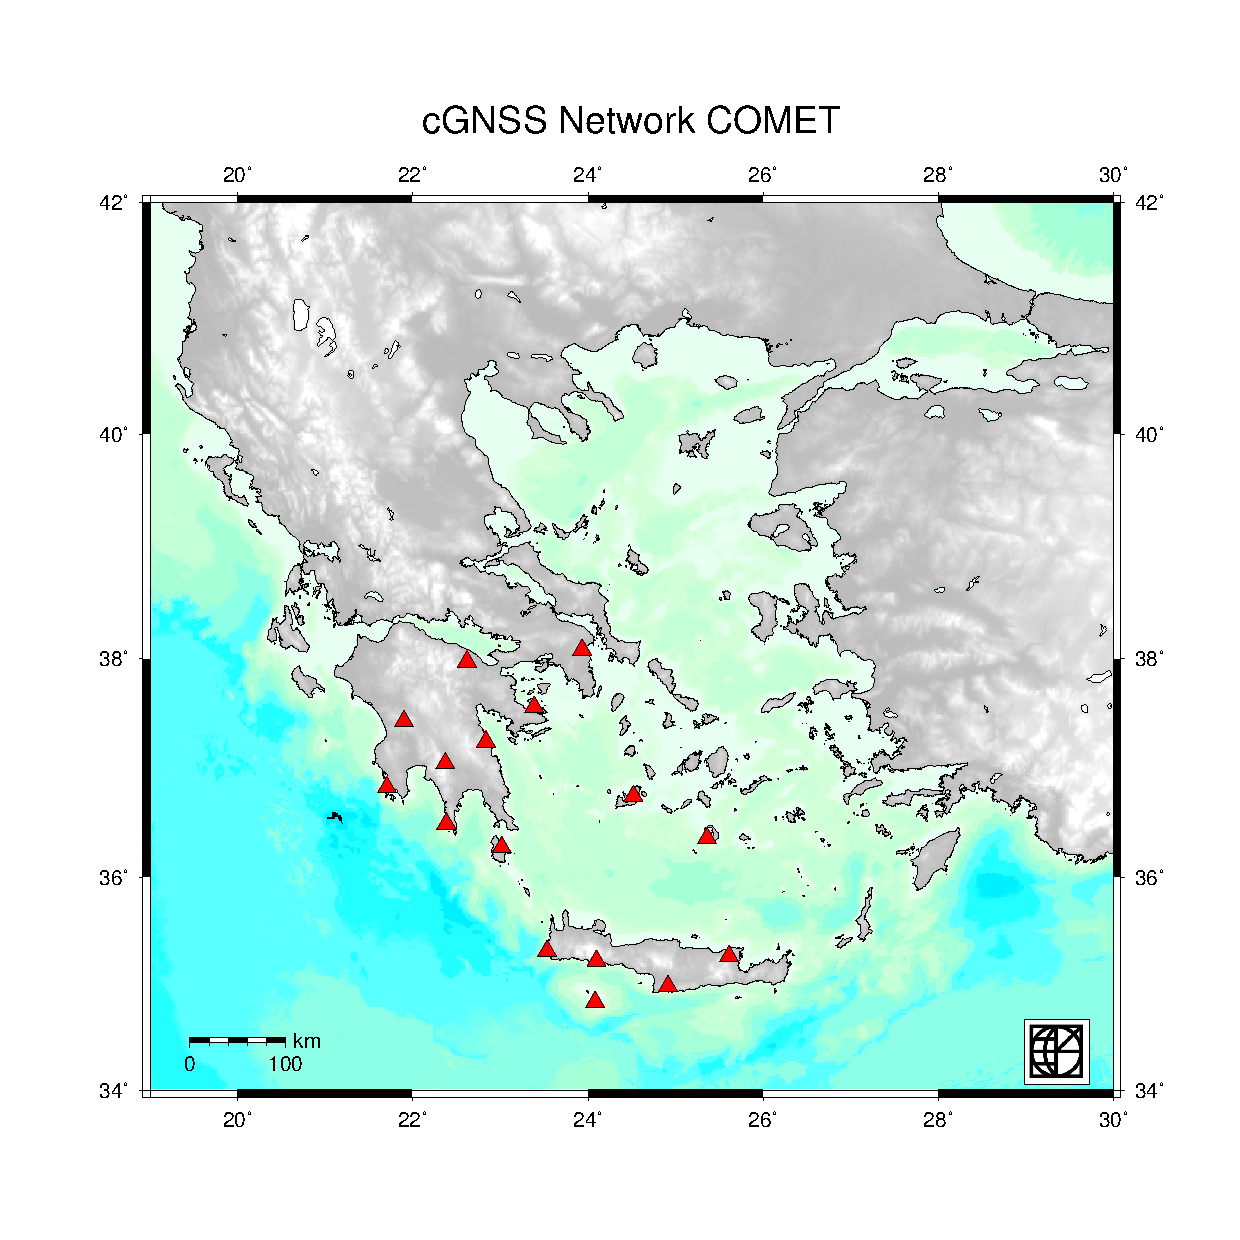
\includegraphics[trim={0cm 2.5cm 0cm 0cm},clip,width=.95\textwidth]{comet.eps} %1 2.2 0 0
 \vskip -.7cm
% \caption{COMET/NTUA network.}
 \label{fig:cometntua}
 \end{center}
 \end{figure}
\end{column}%
\end{columns}
  \begin{block}{}
    Can be used for EUREF densification ``as is''.
  \end{block}
\end{frame}


\begin{frame}\frametitle{Local Networks}\framesubtitle{}
  %Network installed/maintained by \texttt{CRLab}\footnote{Rift Laboratory \url{http://webobs.crlab.eu/}}. 
  \FourQuad
  {
  \textbf{Corinth Rift.}
  \begin{itemize}
    \item<pro@1-> credible time-span
    \item<pro@1-> only covers the Corinth Rift
    \item<con@1-> inconsistent providers
    \item<con@1-> no log files \& equipment changes
  \end{itemize}
  }
  {
 \begin{figure}
 \begin{center}
 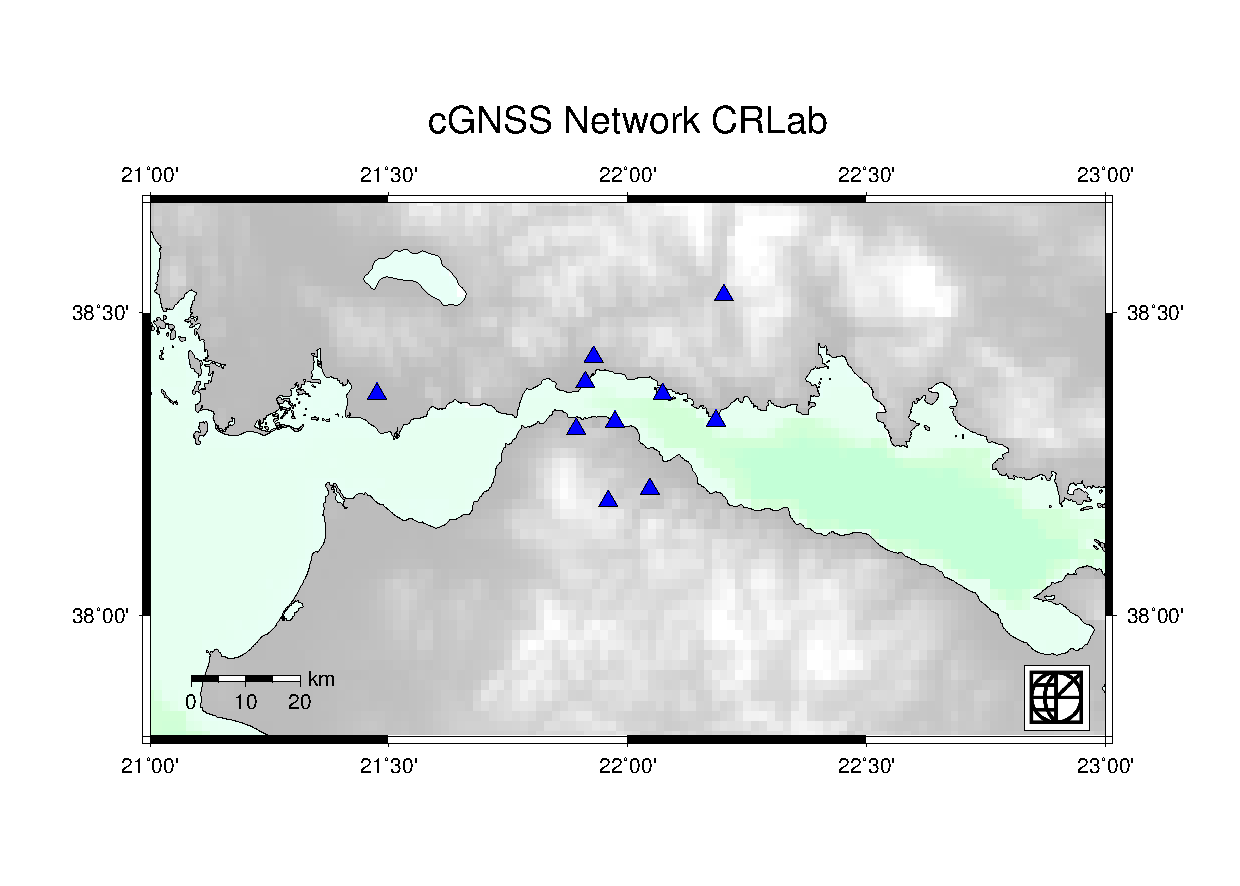
\includegraphics[trim={0cm 2.5cm 0cm 0cm},clip,width=.95\textwidth]{crlnet.eps}
  \vskip -.6cm
 \caption{CRLab network.}
 \label{fig:crlab}
 \end{center}
 \end{figure}
  }
  {
  \textbf{Santorini Network.}
  Most of the stations installed post-2011 to monitor the \textit{inflation episode}.
  \begin{itemize}
    \item<con@1-> localized
    \item<con@1-> limited time-span
  \end{itemize}
  }
  {
 \begin{figure}
 \begin{center}
 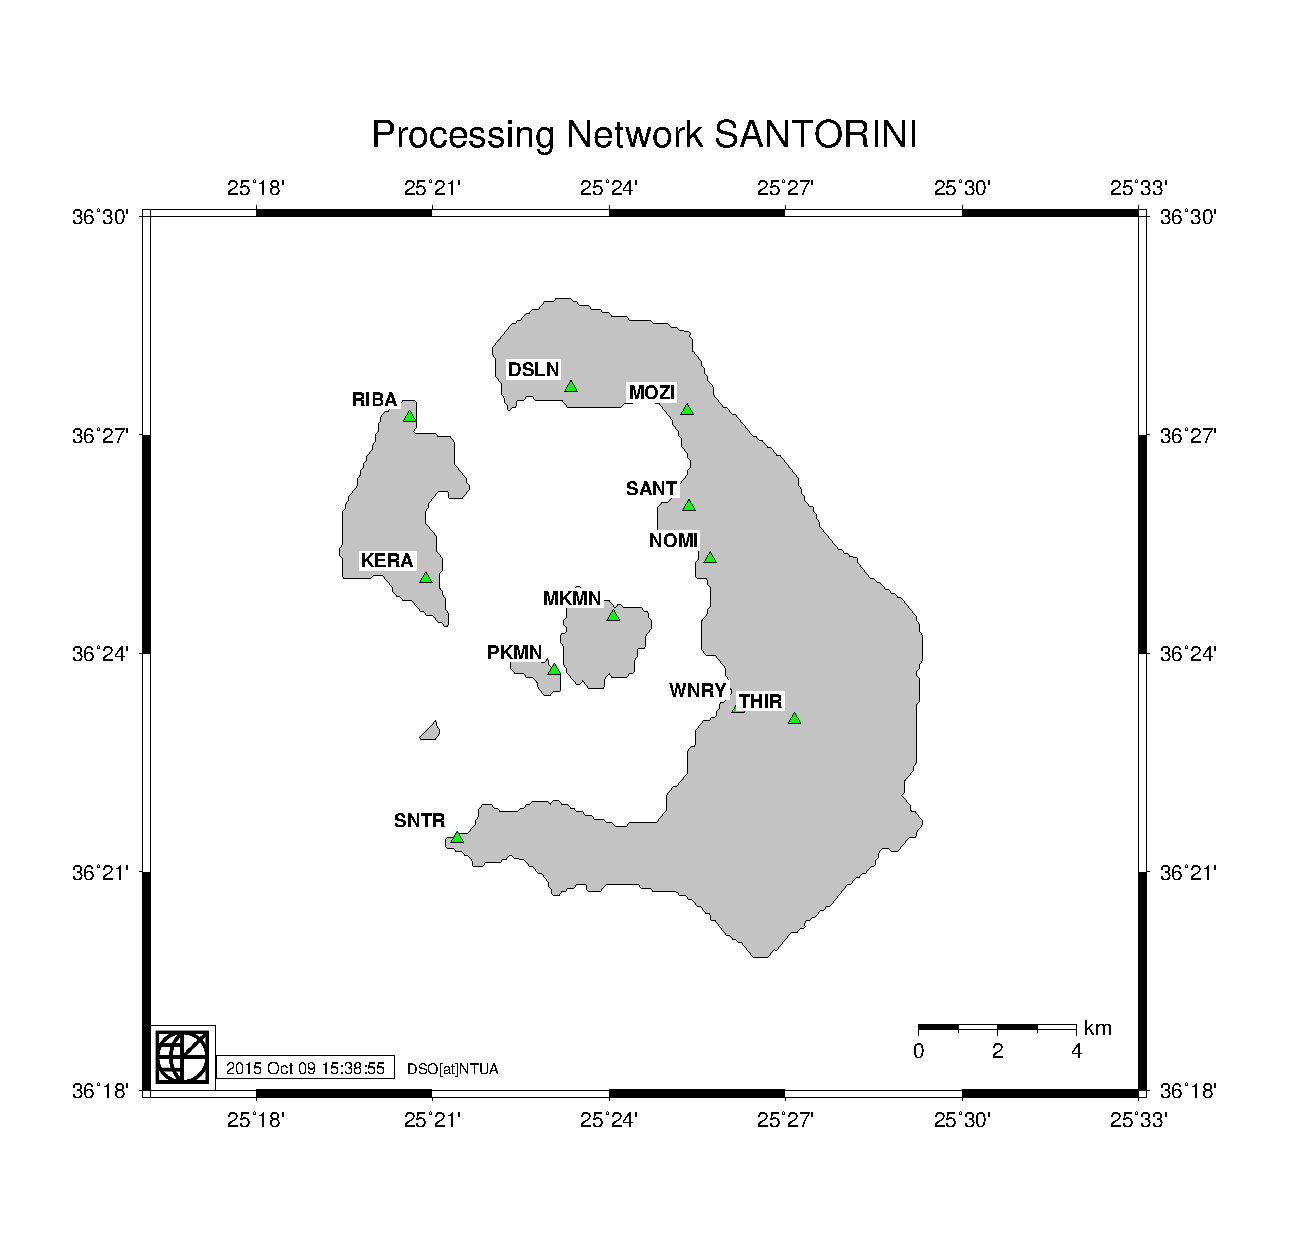
\includegraphics[trim={0cm 2.5cm 0cm 0cm},clip,width=.85\textwidth]{sntrnet.eps}
  \vskip -.6cm
 \caption{Santorini network.}
 \label{fig:sntrnet}
 \end{center}
 \end{figure}
  }
\end{frame}


\section{Processing}

%\begin{frame}\frametitle{The Scheme}\framesubtitle{}
\begin{columns}[T] % align columns
\begin{column}{.28\textwidth}
  The core tool/software is \texttt{Bernese GNSS Software v5.2}\cite{bpe}.\\
  \medskip
  Integration with 
  \begin{itemize}
    \item \texttt{MySQL} database,
    \item \texttt{Python} library
    \item \texttt{GSAC}
    \item wrappers (\texttt{shell})
  \end{itemize}
\end{column}%
\hfill%
\begin{column}{.68\textwidth}
\vskip -1cm
\begin{tikzpicture}[ every annotation/.style = {draw,
                     fill = white, font = \large}]

  \path[mindmap,concept color=black!40,text=white,
    every node/.style={concept,circular drop shadow, scale=.4},
    root/.style = {concept color=black!40,
      font=\normalsize\bfseries,text width=5em},
    level 1 concept/.append style={font=\normalsize\bfseries,
      sibling angle=50,text width=7.7em,
    level distance=20mm,inner sep=0pt},
    level 2 concept/.append style={font=\bfseries,level distance=15mm},
  ]

  node[root] {Bernese GNSS Software v5.2} [clockwise from=0]
    child[concept color=blue!60] {
      node {bernutils Python library} [clockwise from=90]
      child { node[concept] {github repo} }
      child { node[concept] {modules for Bernese output/control files} }
      child { node[concept] {modules for products} }
    }
    child[concept color=blue] {
      node[concept] {MySQL Database} [clockwise from=0]
      child { node[concept] {Bernese .STA} }
      child { node[concept] {IGS log files} }
      child { node[concept] {stations/networks/products} }
    }
    child[concept color=red] {
      node[concept] {/bin wrappers \& utils } [clockwise from=270]
      child { node[concept] {glue everything together} }
      child { node[concept] {various utilities \& formating} }
    }
    child[concept color=yellow!60!black] {
      node[concept] { GSAC } [clockwise from=220]
      child { node[concept] {RINEX} }
      child { node[concept] {products} }
    }
    child[concept color=green!40!black] {
      node[concept] { WebPage } [clockwise from=300]
    }
    \end{tikzpicture}
\end{column}%
\end{columns}
\end{frame}

\begin{frame}\frametitle{Compliance wrt EUREF standards}\framesubtitle{}
  Processing is consistent with EUREFF standards (\href{http://www.epncb.oma.be/_documentation/guidelines/guidelines_analysis_centres.pdf}{Guidelines for Analysis Centres}).
  \begin{itemize}%%[label={\checkmark}]
    \item \texttt{SINEX} with required info/blocks,
    \item Reference frame \texttt{IGb14},
    \item \texttt{IERS} Conventions 2010,
    \item \texttt{IGS}/\texttt{CODE} products,
    \item ocean loading corrections (\texttt{FES2004}),
    \item atmospheric tidal loading corrections,
    \item $3^{\circ}$ elevation cut-off angle; elevation dependent weighting,
    \item \texttt{GMF} and/or \texttt{VMF1}; \texttt{Chen-Herring} gradient parameter,
    \item amiguities fixed (length-dependent algorithm),
    \item use \texttt{GLONASS} obs (when available)
  \end{itemize}
\end{frame}

%  \begin{itemize}
%    \item check station information file consistency (against the provided in \texttt{CODE}'s ftp)
%    \item synchronize \texttt{GEN/} directory
%    \item closely follow \texttt{RNX2SNX.PCF}
%    \begin{itemize}
%      \item variabes in PCF are set by external tools (genericity)
%      \item skip copying/moving/removing; replace with tools that interconnect with \texttt{MySQL}
%    \end{itemize}
%    \item update database
%    \item customize output (\texttt{html, json})
%  \end{itemize}
% \end{frame}

\begin{frame}\frametitle{Workflow}\framesubtitle{}
\begin{columns}[T] % align columns
\begin{column}{.48\textwidth}
  \texttt{\$>ddproces.sh --year= --doy= --session= --bern-loadgps= --campaign= --satellite-system= --solution-id= --save-dir= --analysis-center= --use-ntua-products= --append-suffix= --elevation-angle= --update= --pcv= --apply-exclude-list}
\end{column}
\hfill%
\begin{column}{.48\textwidth}
  \scalebox{0.5}{
  \smartdiagram[priority descriptive diagram]{
    Download \texttt{RINEX} consulting \texttt{MySQL} db,
    Download products,
    Validate \texttt{.STA}; synchronize \texttt{/GEN},
    Set variables in the Protocol Control File (\texttt{.PCF}),
    Process the dataset,
    Check for errors,
    Save Products \& Update database records,
    Compile Report (\texttt{json} | \texttt{html})
}}
\end{column}
\end{columns}
\end{frame}



{
\usebackgroundtemplate{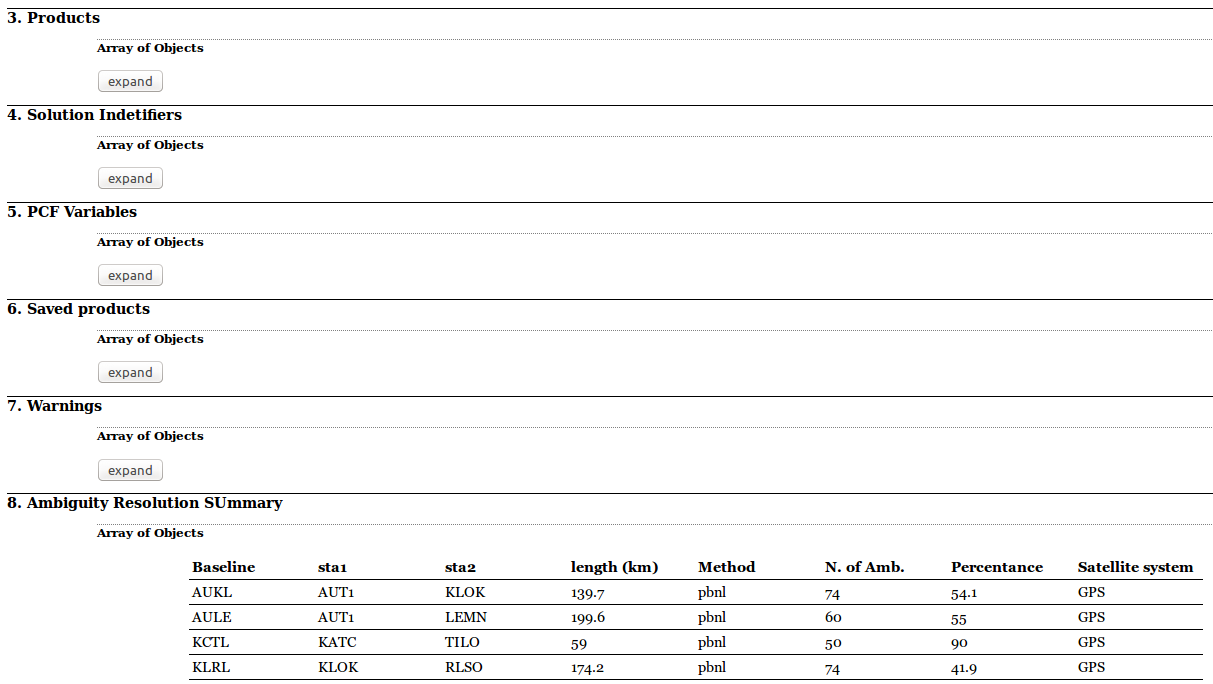
\includegraphics[height=.9\paperheight,width=.9\paperwidth]{jsonprint.png}}
\begin{frame}\frametitle{Results \& Output}\framesubtitle{}
\begin{center}
\vskip -1.6cm
\begin{tikzpicture}
  \node (img1) {\shadowbox{\color{black!35}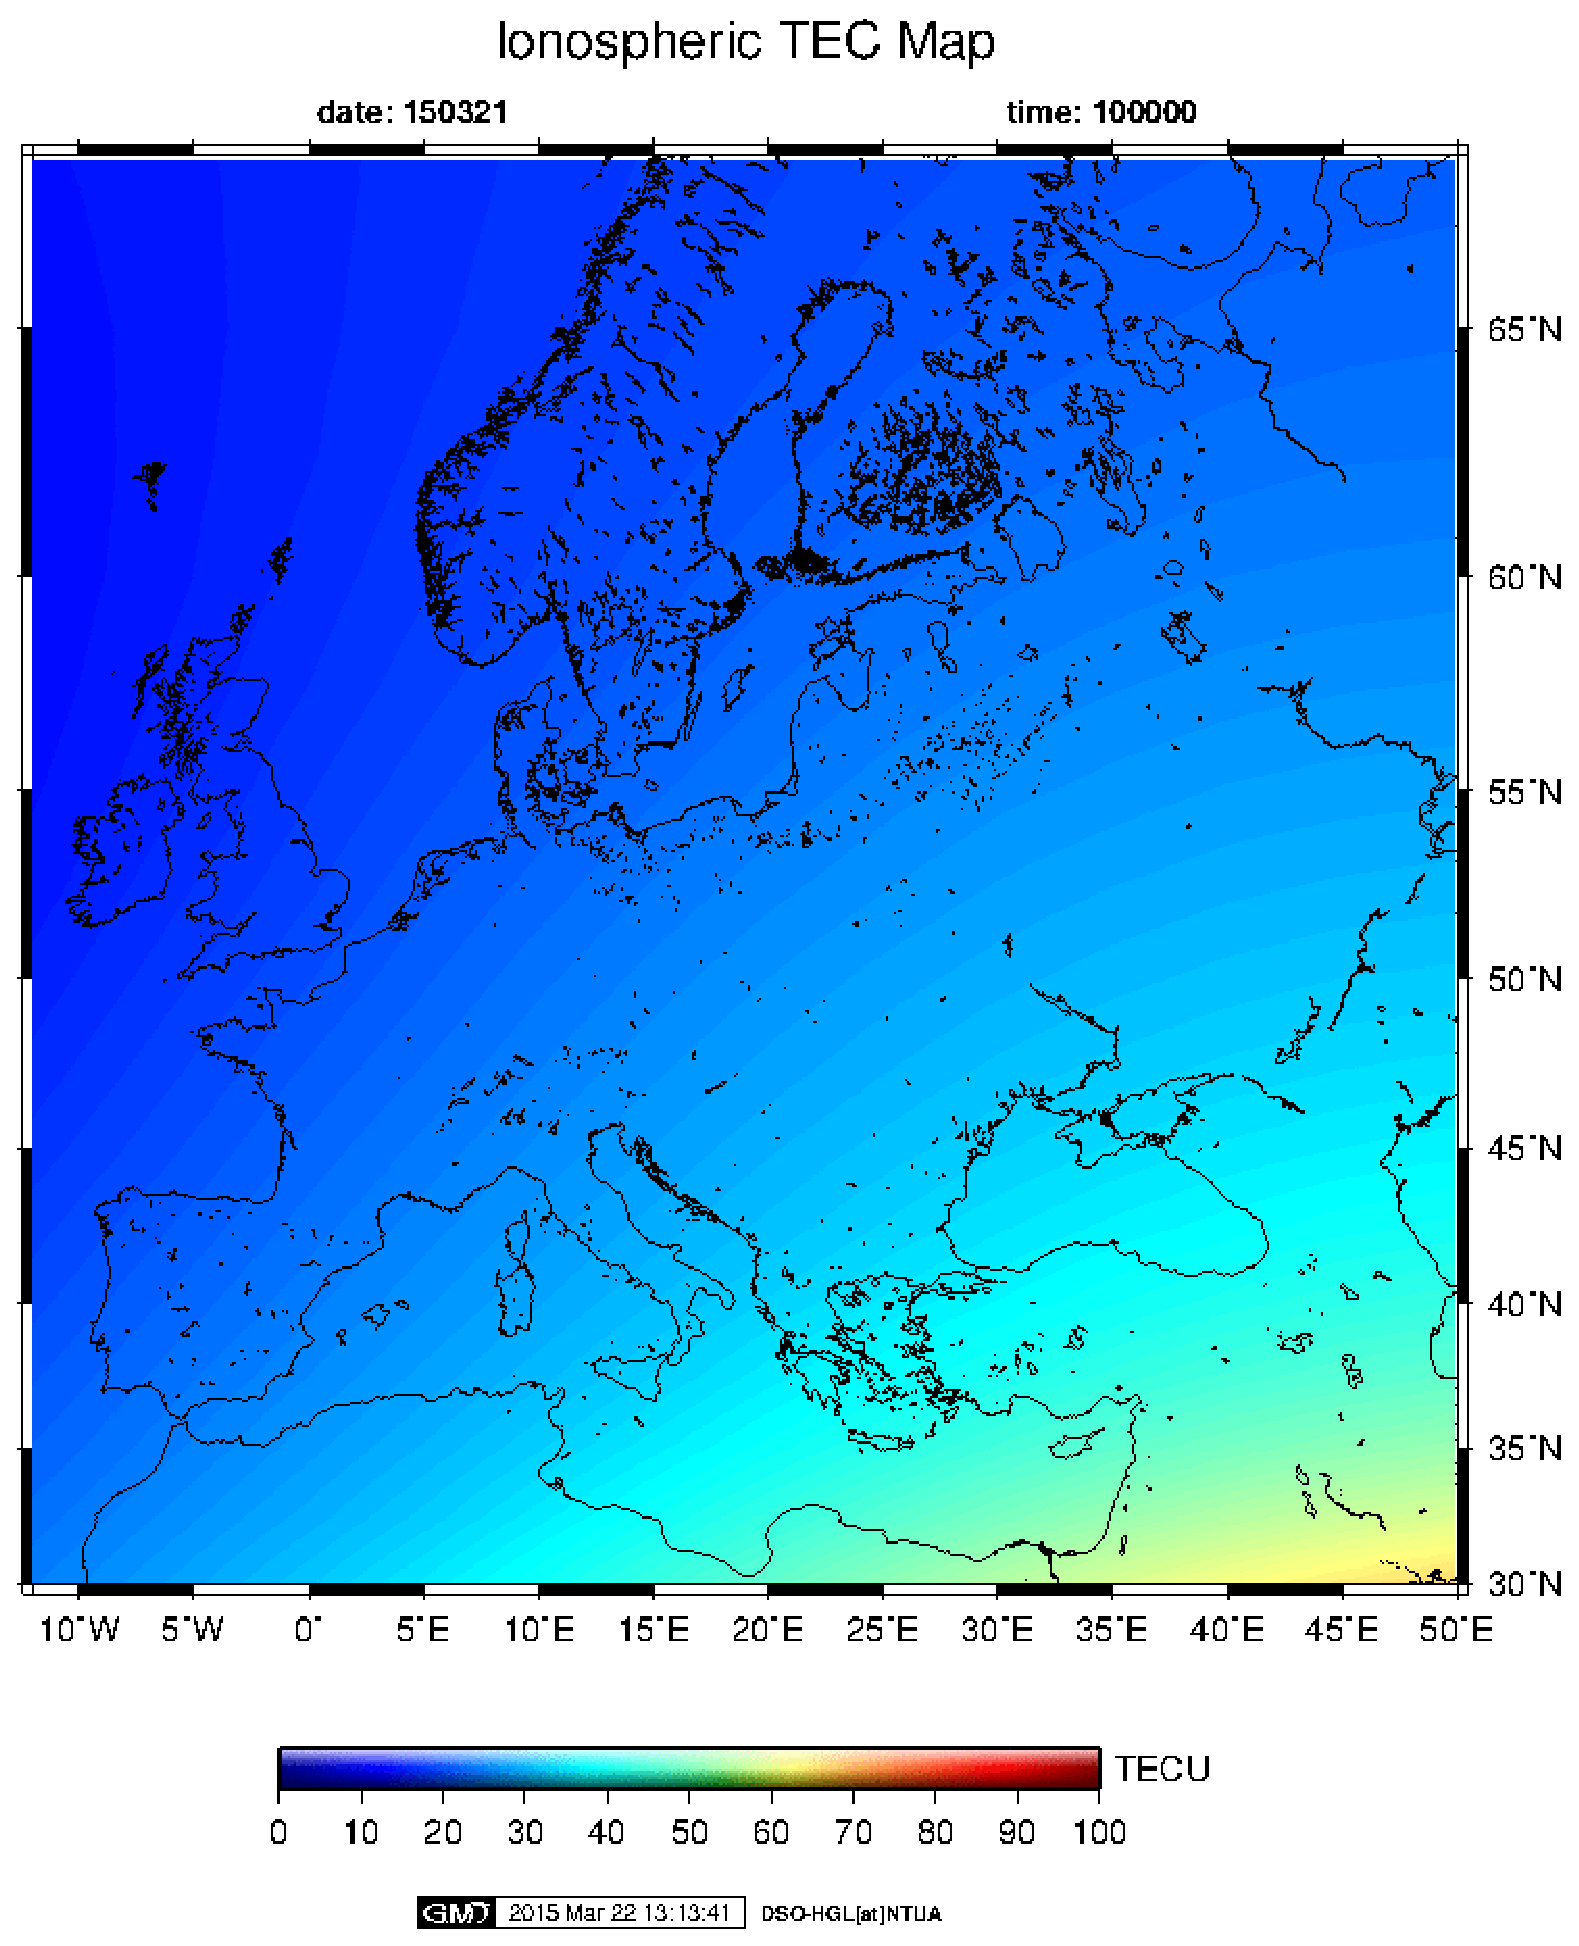
\includegraphics[height=4cm]{iono.eps}}};
%   \pause
  \node (img2) at (img1.north east) [yshift=-1cm,xshift=2.7cm] {\shadowbox{\color{black!35}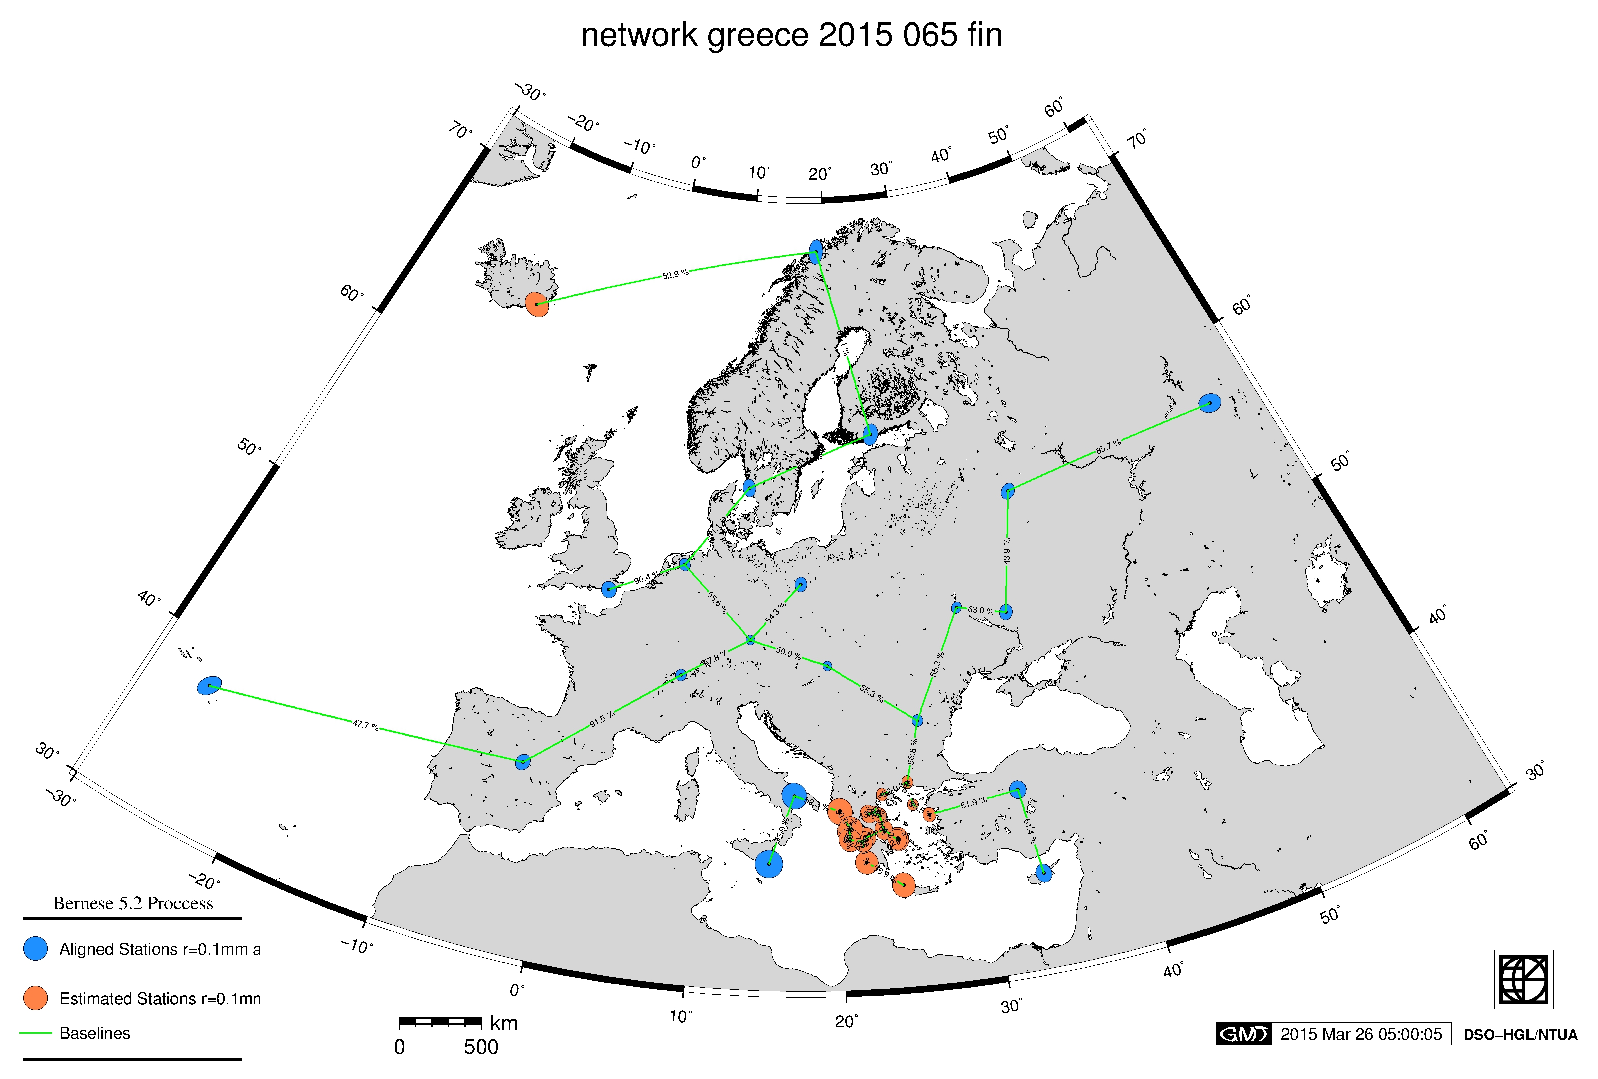
\includegraphics[height=2cm]{baseline.eps}}};
%   \pause
  \node (img3) at (img2.south) [yshift=-1.5cm,xshift=-.5cm] {\shadowbox{\color{black!35}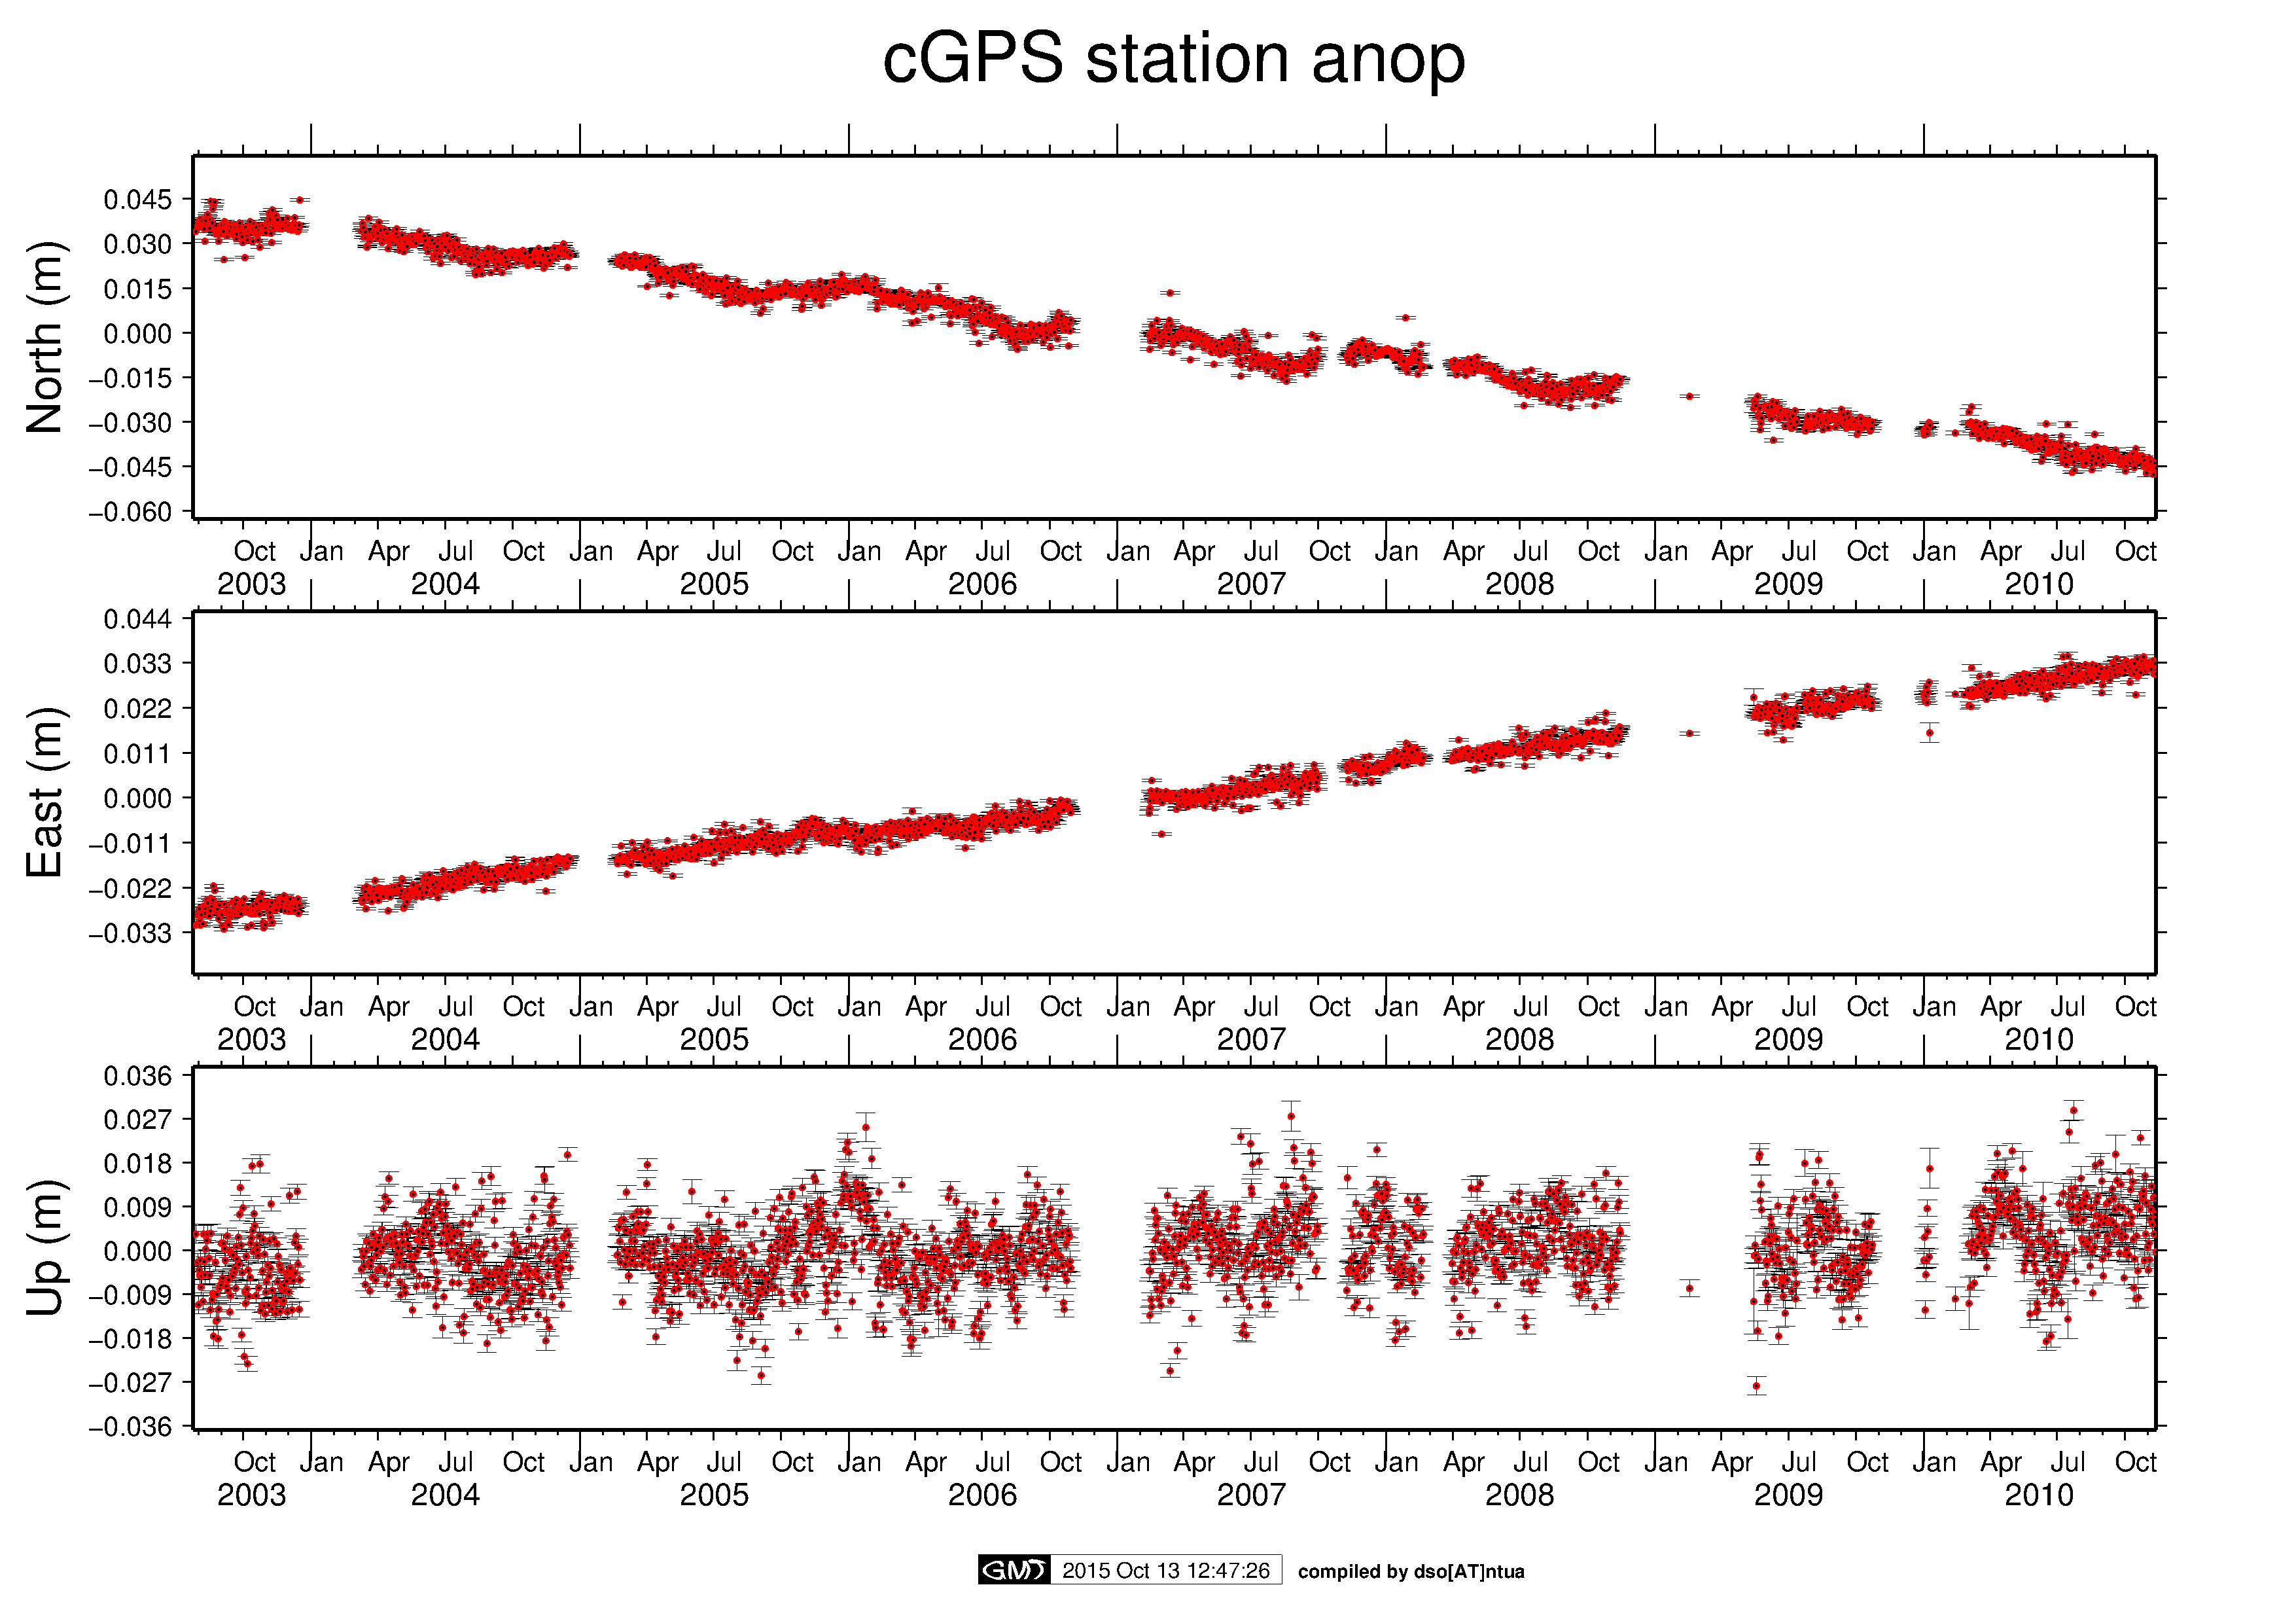
\includegraphics[height=2.6cm]{anop-raw.png}}};
%   \pause
%   \node (img4) at (img2.south west) [yshift=2cm] {\includegraphics[height=4cm]{img/dsoprint.png}};
\end{tikzpicture}
\end{center}
\end{frame}
}






























